\documentclass{article}
\usepackage{graphicx}

\begin{document}
\title{The gaussian error function}
\author{Balazs Doemeny \\ from Wikipedia}
\date{}
\maketitle

\begin{abstract}
\centering
PPNM report
\end{abstract}

\section{Introduction}
In mathematics, the \textbf{error function} (also called the \textbf{Gauss error function}) is a special function (non-Elementary function) of Sigmoid function shape that occurs in probability, statistics, and partial differential equations describing diffusion. It is defined as:


$$
\mathrm{erf}(x)  = \frac{1}{\sqrt{\pi}}\int_{-x}^x e^{-t^2} dt \\
   = \frac{2}{\sqrt{\pi}}\int_0^x e^{-t^2} dt.
$$
In statistics, for nonnegative values of $x$, the error function has the following interpretation: for a random variable $Y$ that is normally distributed with mean 0 and variance 0.5, \textbf{erf($x$)} describes the probability of $y$ falling in the range $[-x,x]$.

\begin{figure}[]
\centering
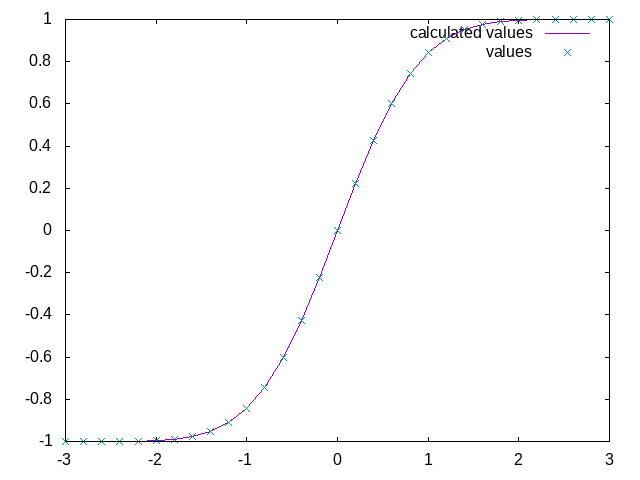
\includegraphics[width=0.7\textwidth]{error_plot.png}
\caption{The error calculated as in the assignment, and in the GSL library}
\end{figure}


There are several closely related functions, such as the complementary error function, the imaginary error function, and others.


\section{Name}


The name "error function" and its abbreviation $erf$ were proposed by J. W. L. Glaisher in 1871 on account of its connection with "the theory of Probability, and notably the theory of Errors". The error function complement was also discussed by Glaisher in a separate publication in the same year. For the "law of facility" of errors whose density is given by $f(x)=\left(\frac{c}{\pi}\right)^{\frac{1}{2}e^{-cx^2}} $ (the normal distribution), Glaisher calculates the chance of an error lying between $p$ and $q$ as:
\begin{equation}
\left(\frac{c}{\pi}\right)^{\frac{1}{2}} \int_p^qe^{-cx^2}dx =\frac{1}{2}\left(\mathrm{erf} (q\sqrt{c}) -\mathrm{erf} (p\sqrt{c})\right)\mathrm{.}
\end{equation}

\section{Applications}

When the results of a series of measurements are described by a  normal distribution with standard deviation  $\sigma$ and expected value $0$, then $\mathrm{erf}\left(\frac{a}{\sigma \sqrt{2}}\right)$  is the probability that the error of a single measurement lies between $-a$ and $+a$, for positive $a$. This is useful, for example, in determining the bit error rate of a digital communication system.

The error and complementary error functions occur, for example, in solutions of the heat equation when boundary conditions are given by the Heaviside step function.

The error function and its approximations can be used to estimate results that hold with high probability. Given random variable $X \sim \mathrm{Norm}[\mu,\sigma]$ and constant $L<\mu$:
\begin{equation}
\mathrm{Pr}[X\leq L] = \frac{1}{2} + \frac{1}{2}\mathrm{erf}\left(\frac{L-\mu}{\sqrt{2}\sigma}\right) \approx A \exp \left(-B \left(\frac{L-\mu}{\sigma}\right)^2\right)
\end{equation}

where $A$ and $B$ are certain numeric constants. If $L$ is sufficiently far from the mean, i.e.   $\mu -L \geq \sigma\sqrt{\ln{k}}$, then:

\begin{equation}
\mathrm{Pr}[X\leq L] \leq A \exp (-B \ln{k}) = \frac{A}{k^B}
\end{equation}

so the probability goes to 0 as $k\rightarrow \infty$.

\section{Values}

\begin{table}[]
%\noindent\hrulefill

\begin{tabular}{|l|l|l|}
\hline
 x & erf(x) & 1-erf(x) \hline \\ \hline
0 & 0  & 1\\ \hline
0.02 & 0.022564575  & 0.977435425\\ \hline
0.04 & 0.045111106  & 0.954888894\\ \hline
0.06 & 0.067621594  & 0.932378406\\ \hline
0.08 & 0.090078126  & 0.909921874\\ \hline
0.1 & 0.112462916  & 0.887537084\\ \hline
0.2 & 0.222702589  & 0.777297411\\ \hline
0.3 & 0.328626759  & 0.671373241\\ \hline
0.4 & 0.428392355  & 0.571607645\\ \hline
0.5 & 0.520499878  & 0.479500122\\ \hline
0.6 & 0.603856091  & 0.396143909\\ \hline
0.7 & 0.677801194  & 0.322198806\\ \hline
0.8 & 0.742100965  & 0.257899035\\ \hline
0.9 & 0.796908212  & 0.203091788\\ \hline
1 & 0.842700793  & 0.157299207\\ \hline
1.1 & 0.88020507  & 0.11979493\\ \hline
1.2 & 0.910313978  & 0.089686022\\ \hline
1.3 & 0.934007945  & 0.065992055\\ \hline
1.4 & 0.95228512  & 0.04771488\\ \hline
1.5 & 0.966105146  & 0.033894854\\ \hline
1.6 & 0.976348383  & 0.023651617\\ \hline
1.7 & 0.983790459  & 0.016209541\\ \hline
1.8 & 0.989090502  & 0.010909498\\ \hline
1.9 & 0.992790429  & 0.007209571\\ \hline
2 & 0.995322265  & 0.004677735\\ \hline
2.1 & 0.997020533  & 0.002979467\\ \hline
2.2 & 0.998137154  & 0.001862846\\ \hline
2.3 & 0.998856823  & 0.001143177\\ \hline
2.4 & 0.999311486  & 0.000688514\\ \hline
2.5 & 0.999593048  & 0.000406952\\ \hline
3 & 0.99997791  & 0.00002209\\ \hline
3.5 & 0.999999257 &  0.000000743 \\ \hline

\end{tabular}

\end{table}

\end{document}
